\documentclass[a4paper, titlepage]{jsarticle}

\date{\today}
\usepackage[dvipdfmx]{graphicx}
\usepackage{url}
% \usepackage[T1]{fontenc}
\usepackage{float}
\usepackage{ascmac}

\title{ドローン宅配事業者支援システム}

\author{土佐山田IT株式会社 \and
        久保田 天治 \and 塩澤 康志 \and 蝉 祐介 \and 寺内 俊輔 \and 林 晃太郎 \and 松本 吏司}

\begin{document}
\maketitle

\tableofcontents

\clearpage

\section{現状の課題}

\section{課題の解決方法}

\section{機能の概要・前提条件・制約事項}

\section{情報・金銭の流れ}

\section{想定する利用者}
本システムが想定する利用者を下記に示す.
\begin{itemize}
        \item 宅配を希望する小規模事業者または個人
        \item 薬を処方する病院または診療所
\end{itemize}

\section{運用・保守}

\section{ハードウェア・ソフトウェアの構成}

\section{費用・効果}

\section{開発体制と工程計画}
本システムの開発は土佐山田IT株式会社の8名により実装する.

本システムの工程計画は図\ref{schedule}に示す.
\begin{figure}[htbp]
        \label{schedule}
        \centering
        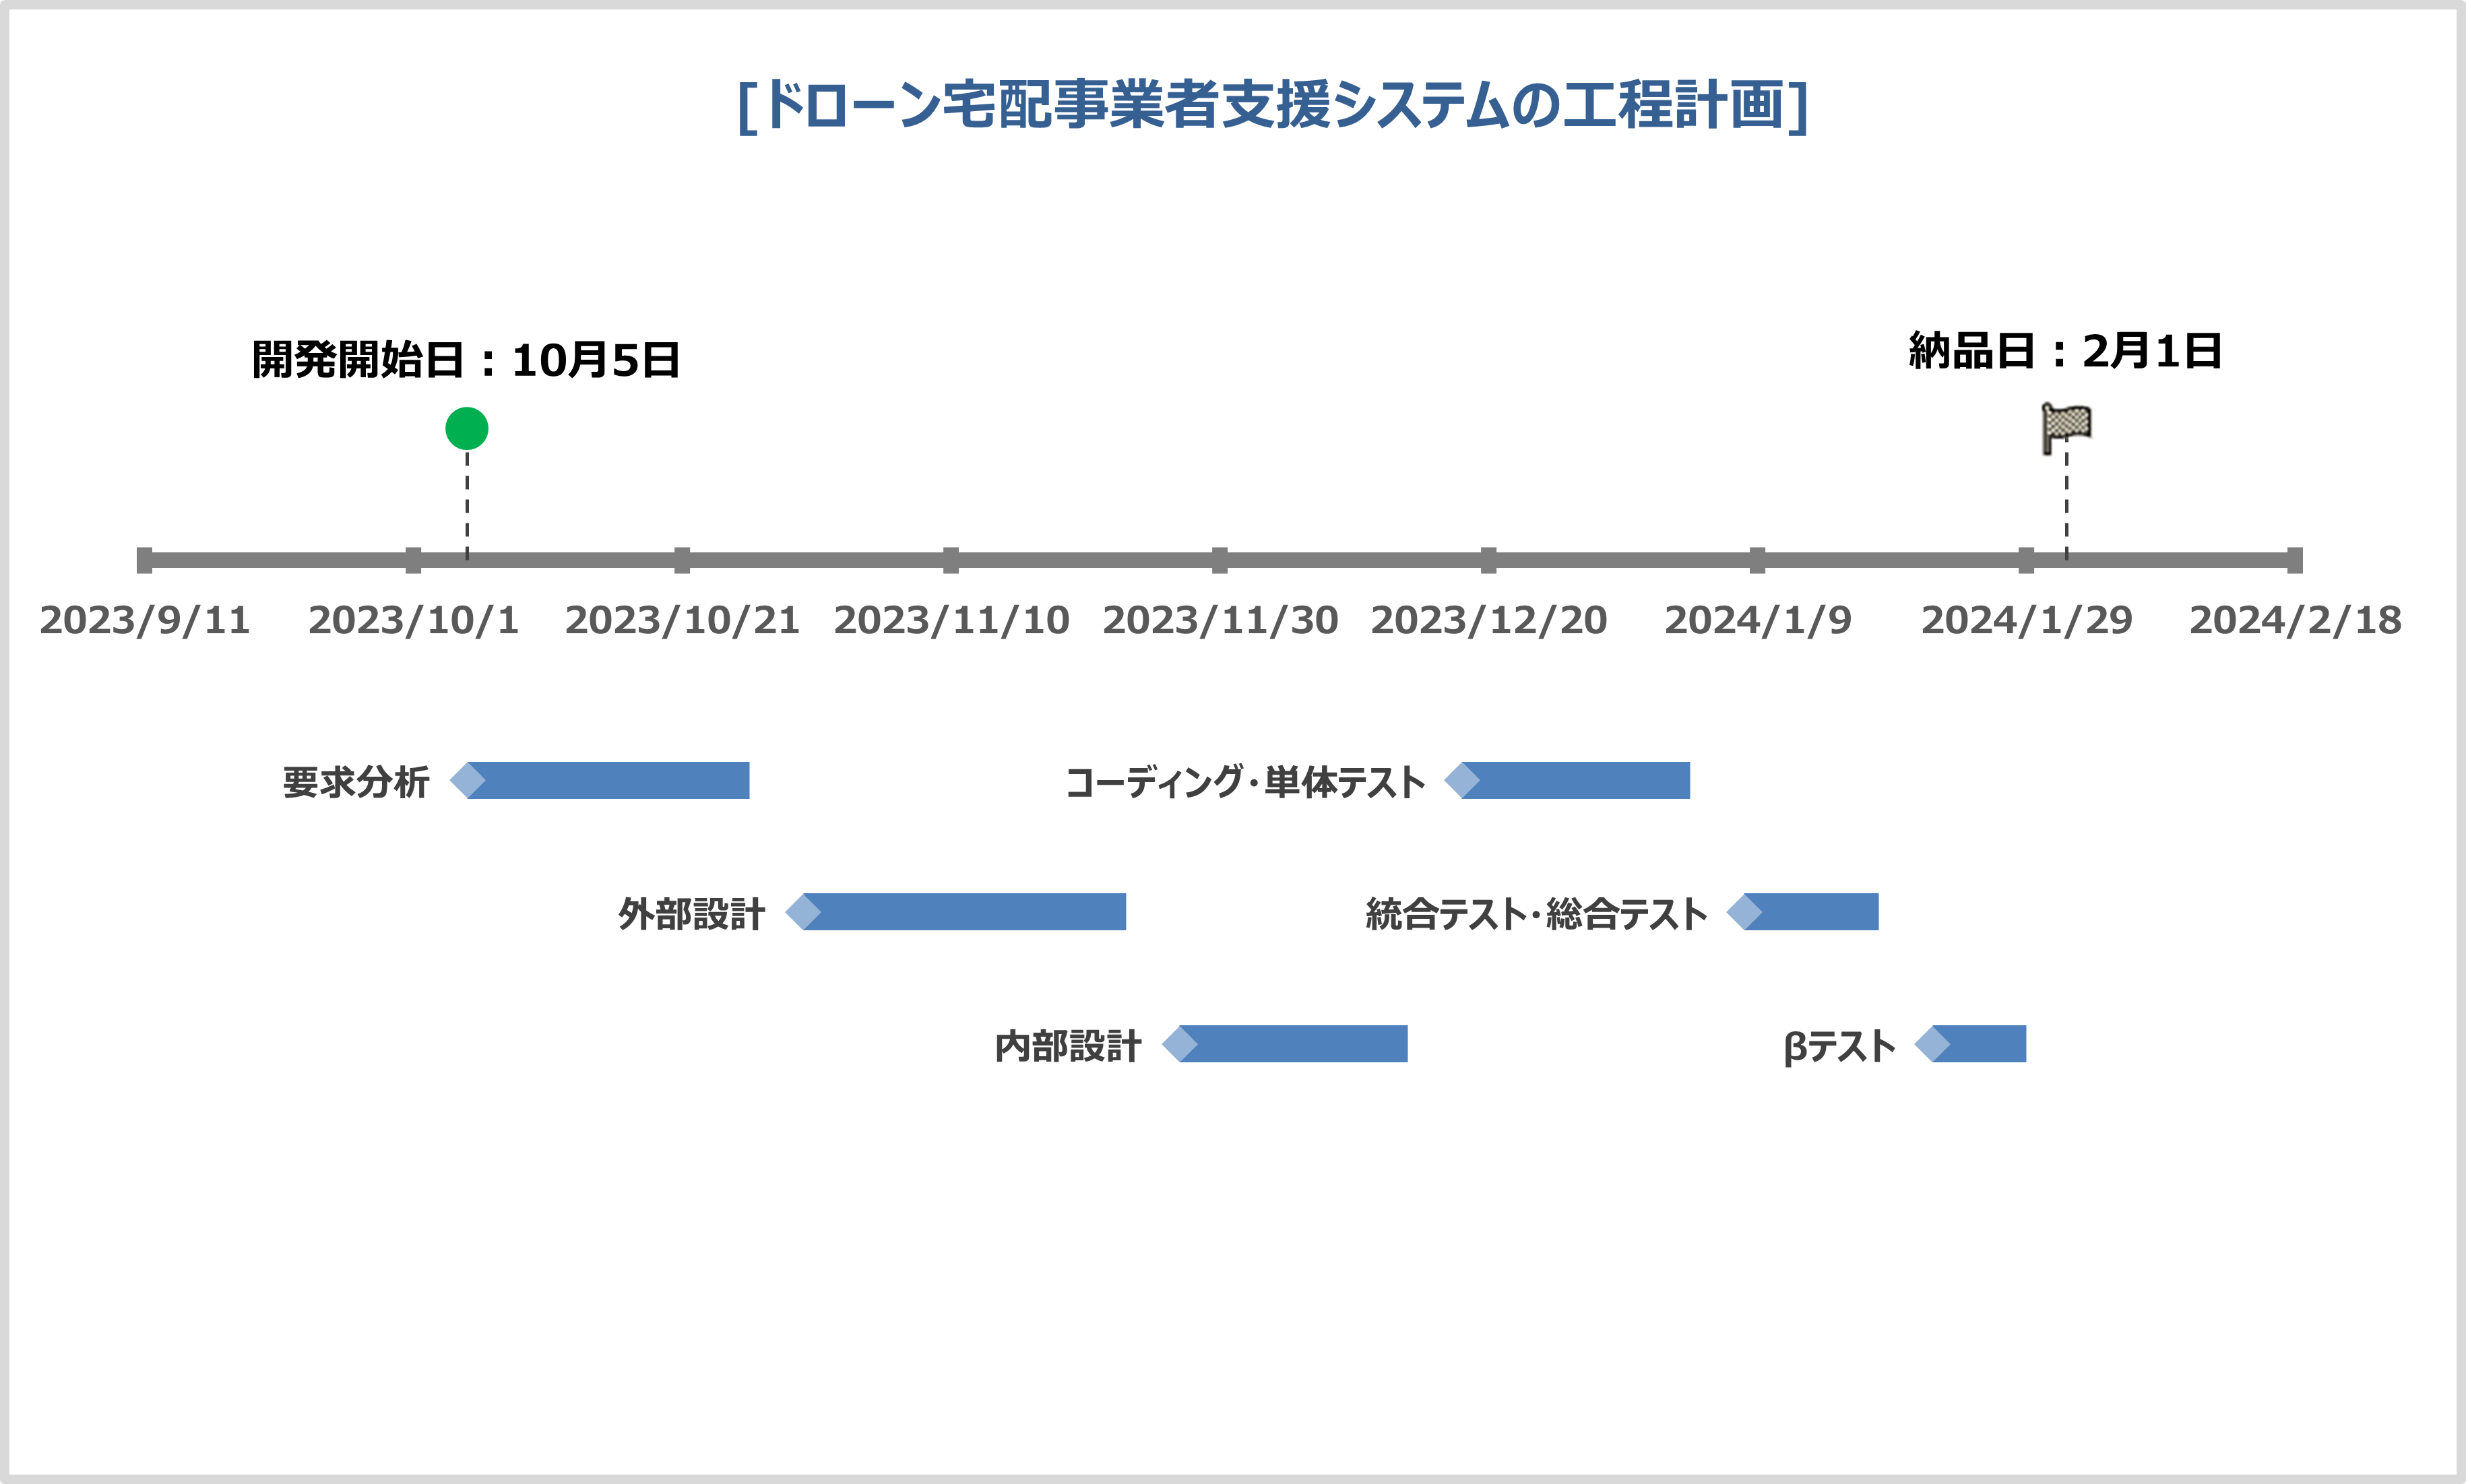
\includegraphics[width=15cm]{schedule.png}
        \caption{工程計画}
\end{figure}

\section{本システムのアピールポイント}
\begin{enumerate}
        \item 未だに日本に存在のしないシステムである.
        \item
\end{enumerate}

\section{貢献度}


\end{document}
